\section{Auswertung}
\label{sec:Auswertung}

\subsection{Bestimmung der freien Weglänge}

Zunächst werden die Sättigungsdampfdrücke $p_\text{sätt}$ aus

\begin{equation*}
p_\text{sätt} = \exp{-\left(\frac{6876}{T}\right)}
\end{equation*}

sowie die mittlere Weglänge der Elektronen aus 

\begin{equation*}
\bar{w}[cm] = \frac{\num{0.0029}}{p_\text{sätt}}[\text{p in mBar}]
\end{equation*}

für die verschiedenen Temperaturen, bei denen die Experimente durchgeführt
werden, bestimmt. Außerdem werden diese Werte mit dem Abstand von $\SI{2}{\centi\meter}$ zwischen Kathode
und Beschleunigungselektrode verglichen. Die Ergebnisse sind in Tabelle \ref{tab:weg} angegeben. 

\begin{table}
  \centering
  \caption{Bestimmung der Sättigungsdampfdrücke, sowie der mittleren Weglängen.}
  \label{tab:weg}
  \sisetup{table-format=2.1}
  \begin{tabular}{c c c c}
  \toprule
  $ T \,/\, \si{\kelvin} $ & $ p_\text{sätt} \,/\, \si{\milli\bar} $ & $\bar{w} \,/\, \si{\centi\meter}$ & $\frac{a}{\bar{w}}$\\
  \midrule 
  296,15 &  0,005 & 0,63895 &     3,13\\
  427,15 &  5,615 & 0,00052 &  3872,46\\
  456,15 & 15,625 & 0,00019 & 10775,68\\
  458,15 & 16,687 & 0,00017 & 11508,61\\
  461,15 & 18,399 & 0,00016 & 12688,94\\
  \bottomrule
  \end{tabular}
  \end{table}

\subsection{Energieverteilung der beschleunigten Elektronen}

Im Folgenden werden die Graphen mit den Titeln 8a) 23°C und 8a) 140°C - 160°C untersucht. Es liegen 
hierbei integrale Energieverteilungen vor. Daher soll zunächst die differentielle Verteilung bestimmt
werden. Die ermittelte Steigung des Graphen 8a) 23°C befindet sich in Tabelle \ref{tab:23}.

\begin{table}
  \centering
  \caption{Ermittelte Steigungen der integralen Elektronenverteilung bei 23°C.}
  \label{tab:23}
  \sisetup{table-format=2.1}
  \begin{tabular}{c c }
  \toprule
  $ U \,/\, \si{\volt} $ & $\frac{\symup{\Delta}y}{\symup{\Delta}x}$\\
  \midrule 
  7,89 & 1,42\\
  8,02 & 2,00\\
  8,11 & 2,50\\
  8,19 & 3,63\\
  8.26 & 3.33\\
  8.32 & 2.38\\
  8.40 & 2.94\\
  8.46 & 1.67\\
  \bottomrule
  \end{tabular}
  \end{table}

Die daraus resultierende differentielle Energieverteilung bei 23°C ist in Abbildung \ref{fig:plot1} zu sehen. 
Die Ordinaten sind dabei proportional zur Anzahl, die Abzissen proportional zur Energie der Elektronen. 

\begin{figure}
  \centering
  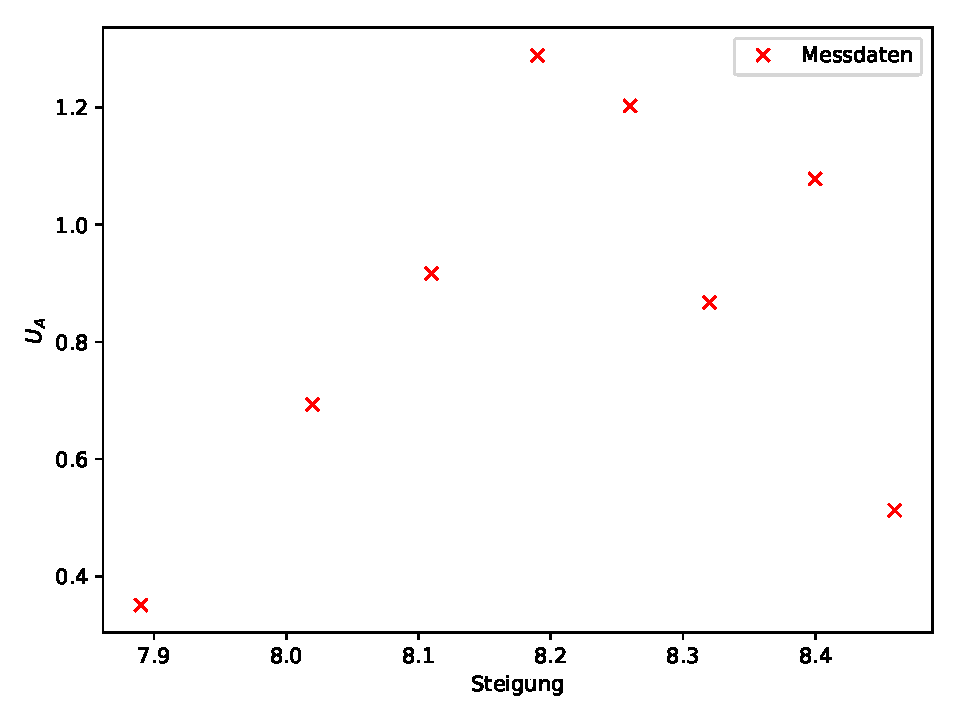
\includegraphics{content/plot1.pdf}
  \caption{Differentielle Energieverteilung bei 23°C.}
  \label{fig:plot1}
\end{figure}

Für den zweiten Graphen wird analog verfahren. Die dazugehörigen Werte befinden sich in Tabelle \ref{tab:154}
und Graph \ref{fig:plot2}.

\begin{table}
  \centering
  \caption{Ermittelte Steigungen der integralen Elektronenverteilung bei 154°C.}
  \label{tab:154}
  \sisetup{table-format=2.1}
  \begin{tabular}{c c }
  \toprule
  $ U \,/\, \si{\volt} $ & $\frac{\symup{\Delta}y}{\symup{\Delta}x}$\\
  \midrule 
  5,32 & 0,550\\
  5,76 & 0,330\\
  6,00 & 0,500\\
  6,16 & 0,625\\
  6,52 & 0,778\\
  6,96 & 0,818\\
  7,36 & 0,800\\
  7,76 & 0,750\\
  8,16 & 0,750\\
  8,56 & 0,700\\
  8,96 & 0,600\\
  9,36 & 0,500\\
  9,76 & 0,400\\
  \bottomrule
  \end{tabular}
  \end{table}

\begin{figure}
  \centering
  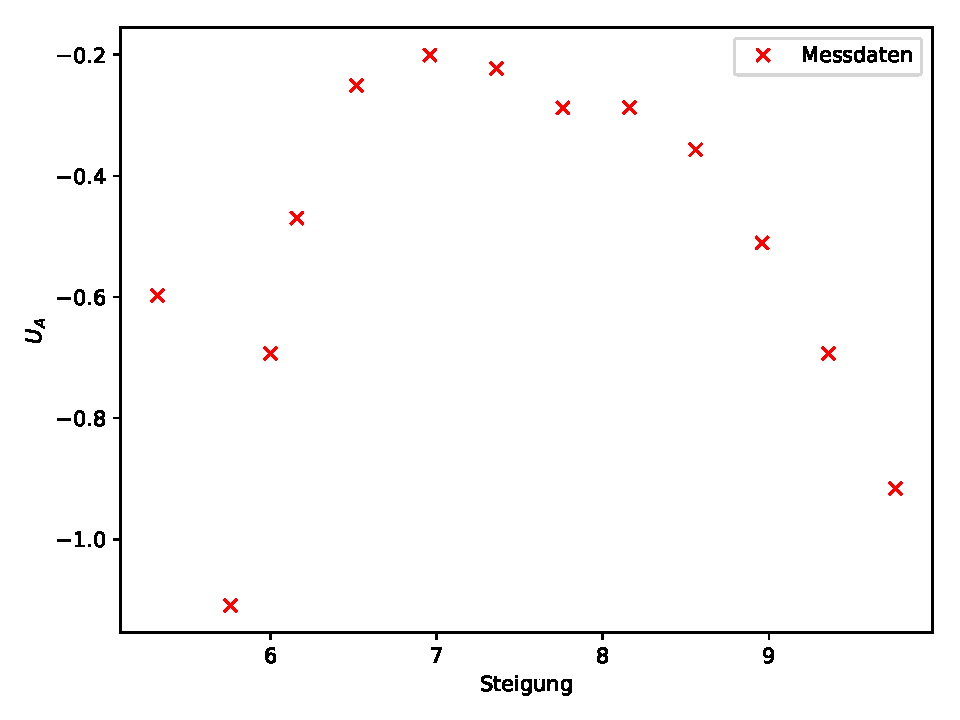
\includegraphics{content/plot2.pdf}
  \caption{Differentielle Energieverteilung bei 154°C.}
  \label{fig:plot2}
\end{figure}

Im ersten Plot ist ein Peak bei $\SI{8.2}{\volt}$ und im zweiten bei $\SI{7}{\volt}$ zu erkennen. 
Das zu bestimmende Kontaktpotential wird für weitere Rechnungen auf 

\begin{equation*}
K_1 = \SI{11}{\volt}-\SI{8.2}{\volt} = \SI{2.8}{\volt}
\end{equation*}

festgelegt. Der Wert von $\SI{11}{\volt}$ ist dabei die angelegte Beschleunigungsspannung.
Eigentlich wird ein einzelner Peak erwartet, der in der Theorie infinitesimal breit ist. In der Praxis 
ist dies offenkundig nicht vorzufinden. Grund dafür ist die Fermi-Dirac-Verteilung. 
Es ist allerdings in Abbildung \ref{fig:plot2} erkennbar, dass bei etwa $\SI{8.2}{\volt}$ ein Abfall der 
Steigung vorliegt. Dies wäre eigentlich bei der Spannung (2.76-2.8)V erwartet worden. Dies ist die Spannung, 
bei der die Elektronen das Quecksilber anregen können minus dem Kontaktpotential. 

\subsection{Anregung des Hg-Atoms}

Mithilfe der aufgezeichneten Franck-Hertz-Kurve soll nun die 1.Anregungsenergie des Hg-Atoms bestimmt 
werden. Dafür wird die Lage der Maxima des Graphen mit dem Titel 8b) 185°C ermittelt, da dieser von
allen aufgenommen Graphen die deutlichsten Maxima und Minima aufweist. Die Maxima und Minima sind mit $k$
nummeriert und mit den jeweiligen Abstände in Tabelle \ref{tab:Max} zu finden. 

\begin{table}
  \centering
  \caption{Abstände der Maxima und Minima der Franck-Hertz-Kurve.}
  \label{tab:Max}
  \sisetup{table-format=2.1}
  \begin{tabular}{c c}
  \toprule
  $k$ & $U_{k+1}-U_{k} \,/\, \si{\volt}$\\
  \midrule 
   1 & 3,04\\
   2 & 2,53\\
   3 & 2,53\\
   4 & 2,53\\
   5 & 2,79\\
   6 & 2,79\\
   7 & 2,53\\
   8 & 2,39\\
   9 & 3,18\\
  10 & 2,79\\
  11 & 3,29\\
  \bottomrule
  \end{tabular}
  \end{table}

Die Abstände müssen mit der Elementarladung multipliziert werden. Es werden sowohl die Maxima, 
als auch die Minima verwendet, um eine höhere Genauigkeit zu erhalten. Es ergibt sich eine 
Anregungsenergie von 

\begin{equation*}
U_1 = \SI{2.76}{\eV}.
\end{equation*}

Aus diesem berechneten Wert wird nun mit Hilfe von $\lambda = \frac{c}{\mu}$ und \eqref{eqn:3} die Wellenlänge
der beim Übergang in den Grundzustand emittierten Strahlung bestimmt werden. Es ergibt sich

\begin{equation*}
\lambda = \SI{273}{\nano\meter}.
\end{equation*}

\subsection{Ionisationsspannung}

Zur Bestimmung der Ionisationsspannung des Quecksilber wird der Graphe mit dem Titel 8c) 107°C verwendet. 
Hierfür wird eine Extrapolation durchgeführt, so wie es in der Abbildung zu sehen ist. Der Schnittpunkt mit 
der x-Achse liegt bei $\SI{8.35}{\volt}$. Mit dem bestimmten Kontaktpotential ergibt sich

\begin{equation*}
U_\text{ion} = \SI{5.55}{\volt}.
\end{equation*}

